\section{Methods}
Methodology: carefully describe the methods you use and why they are appropriate for answering your search questions. It must include
\subsection{Causal Inference}
When studying the relationship between datasets, it is important to distinguish between causation and correlation. While one might find correlations between variables in the data, extra care should be taken before defining causal relationships between the variables. Before making statements on causal relationships, the way the data was generated and any confounders (which may not be captured in the data) must be explored [1]. To ensure that we are not making unsupported claims, we will only seek to find correlation rather than causation in this analysis. 

\subsection{Exploratory Data Analysis}

\begin{figure}
    \centering
    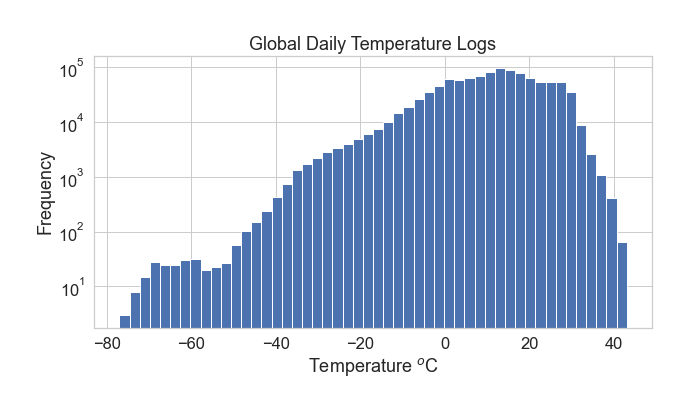
\includegraphics[width=\columnwidth]{figures/DailyTempHist.png}
    \caption{Histogram of daily temeprature logs for all of the stations generated in EDA section of Analysis notebook}
    \label{fig:my_label}
\end{figure}


\subsection{Modeling}
a detailed description of how modeling is done in your project, including inference or prediction methods used, feature engineering and regularization if applicable, and cross-validation or test data as appropriate for model selection and evaluation.
